%\documentclass[12pt,letterpaper,onecolumn]{article}
\documentclass[11pt,letterpaper,onecolumn]{article}
%\documentclass[10pt,letterpaper,onecolumn]{article}  % not recommended
%\documentclass[12pt,letterpaper,twocolumn]{article}
%\documentclass[11pt,letterpaper,twocolumn]{article}
%\documentclass[10pt,letterpaper,twocolumn]{article}


\usepackage{amsmath}
\usepackage{graphicx}
\usepackage{url}
\usepackage{textgreek}
\usepackage{float}
\usepackage{booktabs}
\usepackage{subcaption}
%\graphicspath{{path-to-folder-containing-necessary-graphics}{other folder as necessary}}


%=====================================================
%============ \begin{document} =======================
%=====================================================

\begin{document}

%=====================================================
%============ Title ==================================
%=====================================================

\title{\bf Observation of the Behavior of an B and AB Amplifier}
%\title{\Large\bf Larger, Bolded Title}

%=====================================================
%============ Author =================================
%=====================================================
\author{
 Jairo Portillo \\*
  \\*
 PHY 338K Electronic Techniques \\*
 Department of Physics \\*
 The University of Texas at Austin \\*
 Austin, TX 78712, USA
}
\date{May 6, 2016}

%\address{The University of Texas, Austin, Texas, 78712}

\maketitle

%=====================================================
%============ Abstract ===============================
%=====================================================

\begin{abstract}

In this lab, we will explore the behavior of a class B and class AB push-pull amplifier. The push pull amplifier uses PNP and NPN to amplify the positive and negative portions of a signal respectively. The Class B amplifier causes crossover distortion while the class AB eliminates this distortion with the use of  two diodes.

\end{abstract}

%=====================================================
%============ Body of the article ==========================
%=====================================================

%=====================================================
%============ Section ==================================
%=====================================================

\section{Theory}

 In order to prepare for this lab, we must review the behavior of push pull amplifiers. This amplifier uses both NPN and PNP transistor. The NPN is used in an emitter set up and the PNP is in a follower set up. The NPN emitter cannot sink current and the PNP follower cannon source current. This allows the NPN to amplify the positive portion of the signal while the PNP amplifies the negative portion. This also allows the class B amplifier to have a small voltage gain, yet a much larger power gain and input impedance compared to the output. The Class B is more efficient than a class A as it reduces wasted power by dissipating heat.  
\begin{figure}[H]
    \centering
    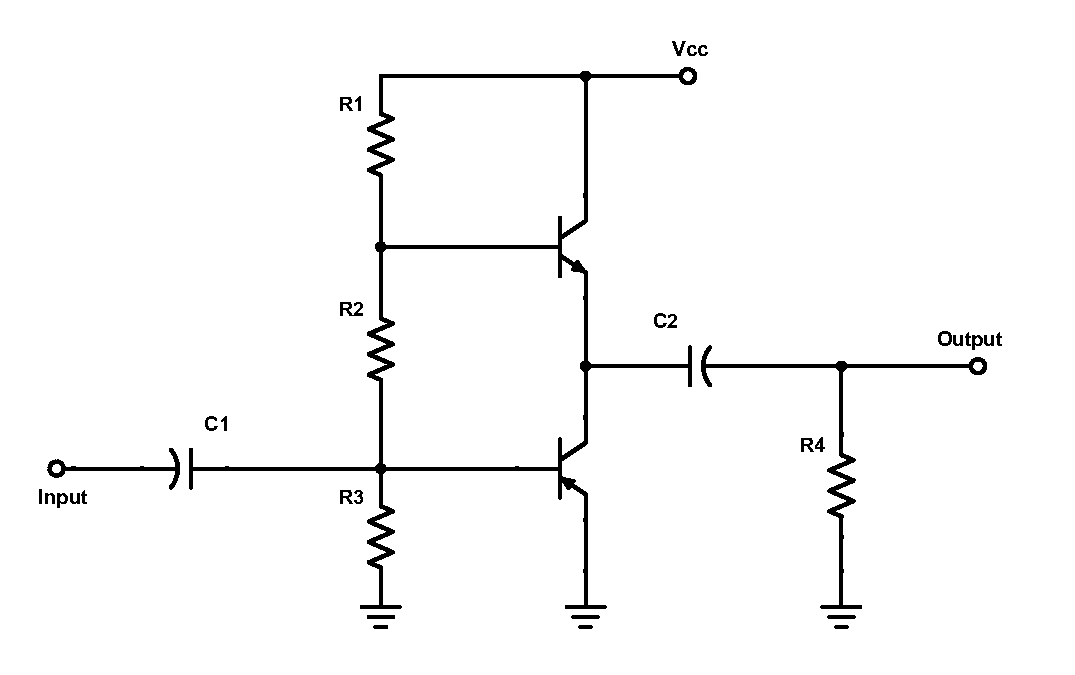
\includegraphics[scale = .7]{lab8cir.pdf}
    \caption{Push Pull Amplifier}
    \label{fig:my_label}
\end{figure}

In a push pull amplifier $R_1 \approx R_3$ within a small error, $R_4 < R_2 < R_1$, $R_4 \ll R_1$, and $C_1 \ll C_2$. Fig 1 is an example of a class B amplifier and a class AB amplifier simply replaces $R_2$ with two forward bias diodes. A disadvantage of the class B is that it produces crossover distortion. This occurs due to the output trailing the input by a $V_{BE}$ drop. The best solution is to use two foward bias diodes producing a class AB amplifier. The diodes introduce a forward voltage drop that compensates for the $V_{BE}$ drop thus allowing the transistors to operate normally. 

\section{Summary and conclusions}

Unfortunately, we were unable to get the class B amplifier to function successfully. We were unable to produce the crossover distortion even with various combinations of $R_1$, $R_2$, $R_3$, and $R_4$ even with $R_2 \ll R_1$. We were able to observe the smooth output with class AB and class B. 


\end{document}